\chapter{Methods}

This chapter will introduce the relevant methodology used in this project. We will introduce two ways how to produce microdroplets, bulk microdroplets, where we use a magnetic stirrer to create microdroplets through rotation and on-chip microdroplets, where we use a microfluidic chip and pressured oil and water phase to create microdroplets. Then we will focus on halo-assays, a method to determine toxicity of antibiotics, used here to screen for potential target of antibiotic producing bacteria. Lastly, we will focus on liquid methodology which helped us to study the problems arising from our setup. We will introduce an experimental setup using conditional medium to study the antibiotic production in liquid.

\section{Bulk droplets}
Droplets can be produced in a flask using a magnetic stirrer and mixing an oil phase with a culture phase~(Figure~\ref{fig:method_droplet_experiments}a). To produce microdroplets in such a way, we mix 70ml of paraffin oil (with an added 2\% of AbilEM90, a surfactant used to guarantee stability of droplets over longer time) with 30ml of~\gls{LB} with added cultured bacteria. Mixing is performed by using a magentic stirrer and slowly increase the stirring speed up to a speed of 600~\gls{rpm}. We keep the stirring constant for 8 minutes before slowly reducing it again. 

\begin{figure}
\centering
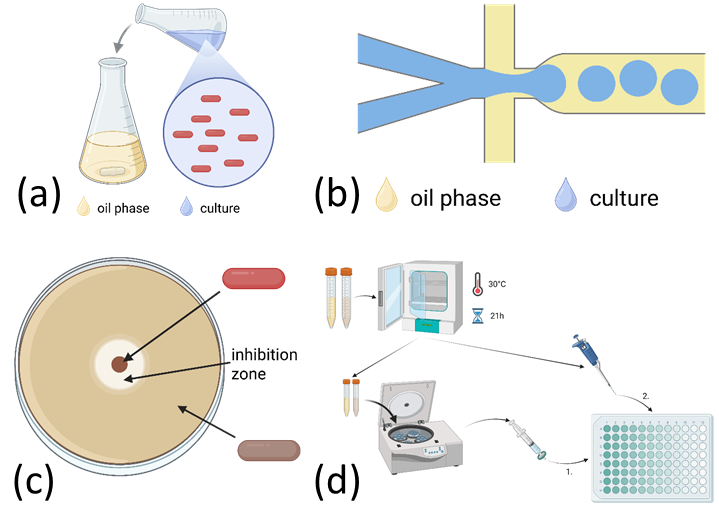
\includegraphics[width=\linewidth]{graphics/2025_09_28_droplets_fig2.png}
\caption{\textbf{Methods used in this project} (a) shows a sketch how to produce bulk micrdroplets. In this method, an oil phase and a bacterial culture are mixed through stirring with a magnetic stirrer. (b) shows a sketch how to produce on-chip microdroplets. In this method, droplets are produced through creating oil and water flows and then creating droplets at a junction inside the microfluidic chip. (c) shows a sketch of a halo assay used to test antibiotic susceptibility. We use this method to find a target strain which is sensitive to the antibiotic produced by our antibiotic producer. In this method, an agar plate is filled with the target strain and small drops of antibiotic or bacteria are placed on top. Forming an inhibition zone indicates if the antibiotic is inhibiting growth. (d) shows a conditional medium assay. We use this assay to check for antibiotic production in liquid. In this method an overnight culture is filtered to remove bacteria and the remaining medium is diluted with fresh medium to create conditional medium. Using a dilution series, we can measure interactions between bacteria, when growing a different strain in this conditional medium.}
\label{fig:method_droplet_experiments}
\end{figure}

\section{On-chip droplets}
Using a commercially available 4-way microfluidic chip (Dolomite), we produce microdroplets. In this method, the oil and water phases are pressurized and flow into a microfluidic chip. Inside the transparent chip the oil and water phase merge at a junction and form water-in-oil microdroplets which are then be collected and incubated~(Figure~\ref{fig:method_droplet_experiments}b). The chip itself does not allow storage of microdroplets inside. We use the same oil and surfactant in this chip as in bulk droplets but we also conducted experiments with Novec\textsuperscript{TM}7500 and added 0.5\% Pico-Surf{\textregistered} (the recommended surfactant).

\section{Halo assay}
We use the well established method of halo assays to screen for possible target starins which are influenced by produced antibiotics. In these assays, we spread $100\mu l$ of the target strain on an LB petri dish and then add drops of $5\mu l$ of the antibiotic producing strain on top of this. After incubation, the target strain grew to a confluent lawn except if the antibiotic is toxic to the target. In that case, an inhibition zone around the drop of producing bacteria is formed. A sketch of the assay is shown in Figure~\ref{fig:method_droplet_experiments}c. Here, the producing bacteria are show in red and the target in brown.  

\section{Liquid and droplet comparison}
To understand how the growth conditions in standard liquid culture and in microdroplets differ, we add to 10ml~\gls{LB} an aliquot  

\section{Conditional medium}